%% --------------------------------------------------------------
%%
%% S T A T I S T I C
%%
%% --------------------------------------------------------------

%% Our models
\newcommand{\DSrefset}{\texttt{M0RefSet}} 
%% large leackage dataset that we usually compare to
\newcommand{\DSheatcool}{\texttt{M0/M1Set}} 
%% all datasets with neutrino absorption
\newcommand{\DScool}{\texttt{LeakSet}}
%% all datasets with leaakge
\newcommand{\DSnone}{\texttt{NoNusSet}}

\def\chid{\chi_{\nu}^2}
\def\non{\nonumber}

%\begin{frame}{Motivation \& Method}
%    \begin{tikzpicture}[overlay,remember picture]
%    \uncover<1->{ % <-> |
%        \node (t1) [anchor=center,scale=1,opacity=1] at ([shift={(-3.6cm,0.5cm)}]current page.center){
%            \parbox{0.60\textwidth}{
%                Link between intrinsic binary parameters \&
%                properties of the EM signal.
%                
%                Fitting formulae to the ejecta and \pmerg{} remnants properties
%        }};
%    }
%
%    \uncover<1->{ % <-> |
%        \node (t1) [anchor=center,scale=1,opacity=1] at ([shift={(-3.6cm,0.5cm)}]current page.center){
%            \parbox{0.60\textwidth}{
%                Compile available NR BNS models into 
%                \DSheatcool{}, \DSrefset{}, \DScool{}, \DSnone{}
%                
%                Assess quality of fits 
%                
%                Fitting formulae to the ejecta and \pmerg{} remnants properties
%        }};
%    }
%
%%    \ac{NR} simulations are the most robust way to obtain the properties of the ejecta
%%
%%    link between the intrinsic binary parameters and properties of the electromagnetic signal.
%%    largest-to-date compiled dataset of \ac{NR} \ac{BNS}
%%    microphysical nuclear \ac{EOS} and neutrino transport.
%%    
%%    growing sample size of \ac{BNS} merger simulations and published ejecta 
%%    properties allow us to asses the dependencies of ejecta and remnant properties on the
%%    binary parameters.
%%    
%%    fitting formulae to the ejecta and \pmerg{} remnants properties of various complexities
%%    
%%    continuous update and reassessment are required as more, higher resolution 
%%    
%%    The motivation for these studies lie in their importance for 
%%    (i) the parameter estimation studies, inferring the binary properties from \ac{EM} observations,
%%    \citep[\eg][]{Radice:2017lry,Perego:2017wtu,Coughlin:2018fis,Coughlin:2019zqi} 
%%    (ii) predicting the properties of the \ac{EM} counterparts from the \ac{GW} observations 
%%    \citep[\eg][]{Stachie:2021noh}, and 
%%    (iii) cosmic chemical evolution models \citep[\eg][]{Bonetti:2019fxj}, as they allow 
%%    to predict how much heavy elements have been injected into \ac{ISM} from mergers.
%    \end{tikzpicture}
%\end{frame}

%% -------------------------------------------------------------------------------------------

\begin{frame}{Motivation \& Method} %% ---------- title 

\begin{tikzpicture}[overlay,remember picture]

\uncover<1->{ % <-> |
    \node (t1) [anchor=center,scale=1,opacity=1] at ([shift={(-3.1cm,1.5cm)}]current page.center){
        \parbox{0.65\textwidth}{
            
            Link between intrinsic binary parameters \&
            properties of the EM signal.
            
            Fitting formulae to the ejecta and \pmerg{} remnants properties
    }};
}
\uncover<1->{ % <-> |
    \node (t1) [anchor=center,scale=1,opacity=1] at ([shift={(-3.1cm,-2.0cm)}]current page.center){
        \parbox{0.65\textwidth}{
            
            Compile $324$ NR BNS models into 
            
            \DSheatcool{}, \DSrefset{}, \DScool{}, \DSnone{} \\
            
            \textbf{Goals} asses
            \begin{itemize}
            \item the quality of fitting formulae (FF), $(\chi_{\nu}^{2})$,
            \item differences between datasets with various physics,
            \item recalibrate all fitting formulae with new data.
            \end{itemize}
            
%            Firring: least square method, minimizing $\chid$
%            \begin{equation*}
%            \chi_{\nu}^{2} = \frac{\chi^2}{N - C} = \frac{1}{N-C}\sum\limits_{i=1}^{N}\Bigg(\frac{o_i - e_i}{o_i ^{\rm err}}\Bigg)^2,
%            \end{equation*}
            
    }};
}

\uncover<1->{ % <-> |
    \node (img1) [anchor=center,scale=1,opacity=1] at ([shift={(5.0cm,-0.2cm)}]current page.center){
        \parbox{0.5\textwidth}{
            \includegraphics[height=6.0cm]{phd_figs/statistics/ej_mej_vej_groups.pdf}
%                \includegraphics[width=0.32\textwidth]{statistics/ej_mej_vej_groups.pdf}
%                \includegraphics[width=0.32\textwidth]{statistics/ej_mej_yeej_groups.pdf}
%                \includegraphics[width=0.32\textwidth]{statistics/ej_vej_yeej_groups.pdf}
%                \caption{Summary of dynamical ejecta properties used in this work.
%                    Blue circles represent models of \DSrefset{}, 
%                    red diamonds stands for models from \DSheatcool{}, 
%                    green crosses are models from \DScool{}
%                    and gray squares stand for models from \DSnone{}, 
%                    %% 
%                    We show for comparison the two-component fit to AT2017gfo as
%                    colored patches from \cite{Villar:2017wcc,Siegel:2019mlp}.
%                    (Adapted from \citet{Nedora:2020qtd})
    }};
}

%Low opacity, fast \ac{SWW} 
%\uncover<1->{ % <-> |
%    \node (t2) [anchor=center,scale=1,opacity=1] at ([shift={(-3.8cm,-1.8cm)}]current page.center){
%        \parbox{0.6\textwidth}{
%            \begin{itemize}
%            \item opservable, related to the remnant lifetime
%            \item probe of remnant dynamics 
%            \end{itemize}
%    }};
%}

\end{tikzpicture}

\end{frame}

%% -------------------------------------------------------------------------------------------

\begin{frame}{Statistical analysis} %% ---------- title 

\begin{tikzpicture}[overlay,remember picture]

\uncover<1->{ % <-> |
    \node (t1) [anchor=center,scale=1,opacity=1] at ([shift={(-3.45cm,-1.0cm)}]current page.center){
        \parbox{0.65\textwidth}{
            We observed
            \begin{itemize}
            \item neutrino raises affects $\amd$, $\avd$
            \item $\tilde{\Lambda}$ \& \mr{} give leading trends
            \item Simple polynomial of them perform well
            \item smooth FFe cannot reproduce well oscillatory data
            \item Correlation between $\avd$ and $\tilde{\Lambda}$ for \DSrefset{}
            %(Higher $\avd$ for $q=1$ models $\rightarrow$ implication for afterglow)
            %Ejecta $\avd$ is reproduced with by datasets with advanced neutrino treatemnt
            \item Statistical analysis of the ejecta geometry (neutrion reabosroption -- more spherical ejecta)
            \item For the disk -- different extraction methods/times
            \end{itemize}
    }};
}

\uncover<1->{ % <-> |
    \node (img1) [anchor=center,scale=1,opacity=1] at ([shift={(4.0cm,0.1cm)}]current page.center){
        \parbox{0.5\textwidth}{
            %\includegraphics[height=6.0cm]{kilonova/mkn_multiband_dyn_NR.pdf}
            %                \includegraphics[width=0.32\textwidth]{statistics/ej_mej_vej_groups.pdf}
            %                \includegraphics[width=0.32\textwidth]{statistics/ej_mej_yeej_groups.pdf}
            %                \includegraphics[width=0.32\textwidth]{statistics/ej_vej_yeej_groups.pdf}
            %                \caption{Summary of dynamical ejecta properties used in this work.
            %                    Blue circles represent models of \DSrefset{}, 
            %                    red diamonds stands for models from \DSheatcool{}, 
            %                    green crosses are models from \DScool{}
            %                    and gray squares stand for models from \DSnone{}, 
            %                    %% 
            %                    We show for comparison the two-component fit to AT2017gfo as
            %                    colored patches from \cite{Villar:2017wcc,Siegel:2019mlp}.
            %                    (Adapted from \citet{Nedora:2020qtd})
            \begin{table}[t]
%            \caption{
%                Reduced $\chi$-squared $\chi^2 _{\nu}$ for different
%                fitting models for the dynamical ejecta properties. Mean is the simulation
%                average, $P_n(x,y)$ is a polynomial of order $n$ in the variables $x,y$. Fits are performed for the data of this work and for an increasingly larger combined dataset from
%                the literature. See text for discussion. 
%                The best fitting model is characterized by the lowest value of $\chi_{\nu}^2$.
%            }
%            \label{tbl:fit:ejecta:chi2dofsall}
            \scalebox{0.55}{
                \begin{tabular}{l|l|ccccc}
                \hline\hline
                $\log_{10}(\md)$ & Datasets & Mean & Eq.~\eqref{eq:fit_Mej} & Eq.~\eqref{eq:fit_Mej_Kruger} & $P_2^1(\tilde{\Lambda})$ & $P_2^2(q,\tilde{\Lambda})$ \\ \hline
                & \DSrefset{} & 3.84 & 2.23 & 1.58 & 3.03 & 1.55 \\ 
                & \& \DSheatcool{}  & 26.66 & 16.85 & 10.60 & 37.29 & 56.45 \\ 
                & \& \DScool{}  & 99.11 & 30.12 & 11.91 & 45.59 & 24.40 \\ 
                & \& \DSnone{}  & 196.52 & 84.81 & 39.88 & 123.56 & 44.36 \\ 
                \hline\hline
                $\langle v_{\rm ej}\rangle$ & Datasets & Mean & Eq.~\eqref{eq:fit_vej} & & $P_2^1(\tilde{\Lambda})$ & $P_2^2(q,\tilde{\Lambda})$ \\ \hline
                & \DSrefset{} & 3.76 & 1.51 & & 3.24 & 1.05 \\ 
                & \& \DSheatcool{}  & 4.03 & 2.42 & & 3.35 & 1.67 \\ 
                & \& \DScool{}  & 7.10 & 6.07 & & 6.34 & 5.09 \\ 
                & \& \DSnone{}  & 7.95 & 6.79 & & 7.64 & 6.83 \\ 
                \hline\hline
                $\langle Y_{\rm e}\rangle$ & datasets & Mean &  & & $P_2^1(\tilde{\Lambda})$ & $P_2^2(q,\tilde{\Lambda})$ \\ \hline
                & \DSrefset{} & 42.49 &  & & 43.69 & 9.07 \\ 
                & \& \DSheatcool{}  & 37.78 &  & & 38.62 & 9.68 \\ 
                & \& \DScool{}  & 35.80 &  & & 36.27 & 24.96 \\ 
                \hline\hline
                $\langle \theta_{\rm RMS}\rangle$ & datasets & Mean & & & $P_2^1(\tilde{\Lambda})$ & $P_2^2(q,\tilde{\Lambda})$ \\ \hline
                & \DSrefset{} & 20.68 & & & 21.66 & 4.55 \\ 
                & \& \DSheatcool{}  & 18.18 & & & 18.69 & 4.17 \\ 
                & \& \DScool{}  & 15.56 & & & 14.34 & 8.73 \\ 
                \hline\hline
                \end{tabular}
            }%scalebox
            \end{table}
    }};
}

%Low opacity, fast \ac{SWW} 
%\uncover<1->{ % <-> |
%    \node (t2) [anchor=center,scale=1,opacity=1] at ([shift={(-3.8cm,-1.8cm)}]current page.center){
%        \parbox{0.6\textwidth}{
%            \begin{itemize}
%            \item opservable, related to the remnant lifetime
%            \item probe of remnant dynamics 
%            \end{itemize}
%    }};
%}

\end{tikzpicture}

\end{frame}
